
\documentclass[a4paper,12pt]{article}

\usepackage[margin=1.5cm]{geometry}
\usepackage[T1]{fontenc}
\usepackage{lmodern}
\usepackage{tikz}

\pagestyle{empty}

\begin{document}

\begin{center}
    {\Large\bfseries UML Class Diagram}\\[4pt]
    {\large LeaveRequest Class}
\end{center}

\vspace{0.8cm}

\begin{center}
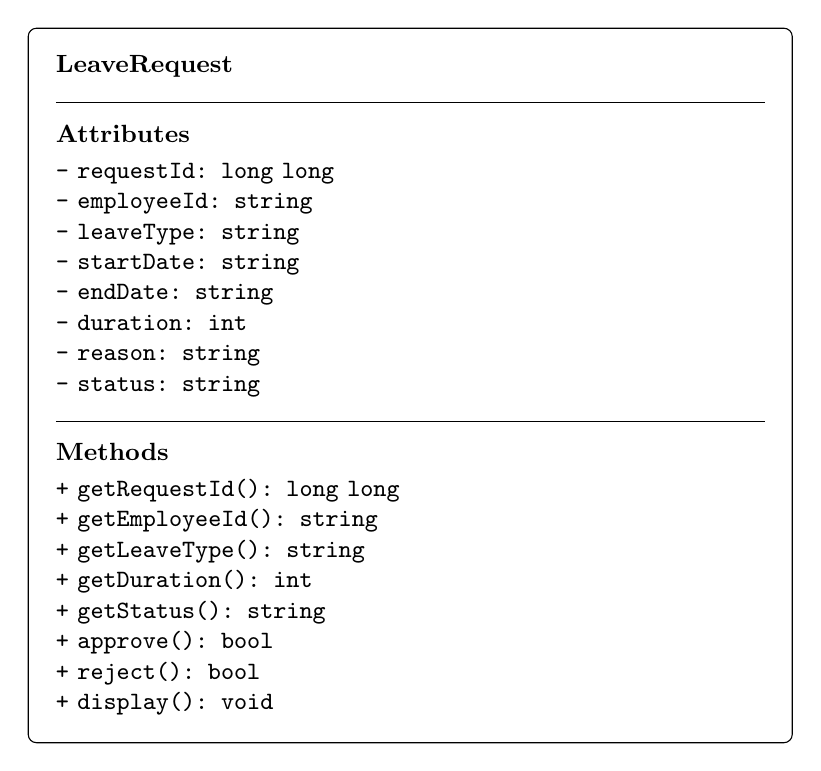
\begin{tikzpicture}[
    classbox/.style={
        draw,
        rounded corners=3pt,
        align=left,
        text width=9cm,
        inner sep=10pt,
        font=\small
    }
]

\node[classbox] (request) {
    \textbf{LeaveRequest}\\
    \rule{\linewidth}{0.4pt}\\[3pt]
    \textbf{Attributes}\\[2pt]
    \texttt{- requestId: long long}\\
    \texttt{- employeeId: string}\\
    \texttt{- leaveType: string}\\
    \texttt{- startDate: string}\\
    \texttt{- endDate: string}\\
    \texttt{- duration: int}\\
    \texttt{- reason: string}\\
    \texttt{- status: string}\\
    \rule{\linewidth}{0.4pt}\\[3pt]
    \textbf{Methods}\\[2pt]
    \texttt{+ getRequestId(): long long}\\
    \texttt{+ getEmployeeId(): string}\\
    \texttt{+ getLeaveType(): string}\\
    \texttt{+ getDuration(): int}\\
    \texttt{+ getStatus(): string}\\
    \texttt{+ approve(): bool}\\
    \texttt{+ reject(): bool}\\
    \texttt{+ display(): void}
};

\end{tikzpicture}
\end{center}

\vspace{0.6cm}

\noindent
\textbf{Description:}
The \texttt{LeaveRequest} class represents an employee's leave
application. It stores the request details and status, provides
getter methods, and supports approval and rejection operations.

\end{document}
